Para esta sección se consideran las señales $x_1(t) = \sin{(\omega t)}$, $x_2(t) = \cos{(\omega t)}$, ambas con frecuencia 100 Hz y muestreadas a $f_s = 5~kHz$ durante $100~ms$.

\begin{enumerate}
    \item Se pide obtener expresiones analíticas para las DTFT de las señales muestreadas $x_1[n],~ x_2[n]$, considerando duración infinita y los 100 ms.
    
    \textbf{DTFT de $x_1(n)$ de duración infinita:}
    
    En primer lugar se obtiene la versión muestreada de la señal en el dominio temporal:
    $$ x_1[n] = \sin{(2\pi f/f_s~n)} =  \sin{(0.04\pi n)} = \sin{(\omega_0 n)}$$
    
    Luego la DTFT está dada por:
\begin{align*}
    X_1(\omega) &= \sum_{n=-\infty}^{\infty}x_1[n]e^{-j\omega n}\\
    &= \sum_{n=-\infty}^{\infty}\sin{(\omega_0 n)}e^{-j\omega n}\\
    &= \sum_{n=-\infty}^{\infty}\left(\dfrac{e^{j\omega_0n} - e^{-j\omega_0n} }{2j}\right)e^{-j\omega n}\\
    &= \dfrac{1}{2j}\left(\sum_{n=-\infty}^{\infty}e^{j\omega _0n}e^{-j\omega n} - \sum_{n=-\infty}^{\infty}e^{-j\omega_0 n}e^{-j\omega n}\right)\\
    &= \dfrac{1}{2j}\left(2\pi\delta(\w-\w_0) - 2\pi\delta(\w+\w_0)\right)\\
    &= \dfrac{\pi\delta(\w-\w_0) - \pi\delta(\w+\w_0)}{j}\\
\end{align*}

    Cabe destacar que la expresión obtenida considera $\w \in [-\pi, \pi] $, si se desea para todo $\w$ debe considerarse periodicidad de periodo $2\pi$ del espectro en frecuencia.
    
    \textbf{DTFT de $x_2(n)$ de duración infinita:}
    
    Se obtiene la versión muestreada de la señal en el dominio temporal:
    $$ x_2[n] = \cos{(2\pi f/f_s~n)} =  \cos{(0.04\pi n)} = \cos{(\omega_0 n)}$$
    
    Luego la DTFT está dada por:
\begin{align*}
    X_2(\omega) &= \sum_{n=-\infty}^{\infty}x_2[n]e^{-j\omega n}\\
    &= \sum_{n=-\infty}^{\infty}\cos{(\omega_0 n)}e^{-j\omega n}\\
    &= \sum_{n=-\infty}^{\infty}\left(\dfrac{e^{j\omega_0n} + e^{-j\omega_0n} }{2}\right)e^{-j\omega n}\\
    &= \dfrac{1}{2}\left(\sum_{n=-\infty}^{\infty}e^{j\omega _0n}e^{-j\omega n} + \sum_{n=-\infty}^{\infty}e^{-j\omega_0 n}e^{-j\omega n}\right)\\
    &= \dfrac{1}{2}\left(2\pi\delta(\w-\w_0) + 2\pi\delta(\w+\w_0)\right)\\
    &= \pi\delta(\w-\w_0) + \pi\delta(\w+\w_0)\\
\end{align*}

    Cabe destacar que la expresión obtenida considera $\w \in [-\pi, \pi] $, si se desea para todo $\w$ debe considerarse periodicidad de periodo $2\pi$ del espectro en frecuencia.
    
    \textbf{DTFT de $x_1[n]$:}
    
    Debido a que $x_1[n]$ corresponde a la señal de duración infinita multiplicada por una ventana cuadrada, se obtiene su DTFT como la convolución de el espectro de la señal de duración infinita y el espectro de la ventana cuadrada $W(e^{j\w})$
    
    El espectro de la ventana está dado por:
    $$W(e^{j\omega}) = e^{-j\omega(N-1)/2}\dfrac{\sin{(\omega N}/2)}{sin(\w/2)}$$
    donde $N=500$ ya que la ventana de 100 ms es de 500 muestras.
    
    Luego el espectro de la señal enventanada está dado por:
    \begin{align*}
       X_1^{(w)}(\w) &= X_1(\w) \ast W(e^{j\omega})\\
       &= \left(\dfrac{\pi\delta(\w-\w_0) - \pi\delta(\w+\w_0)}{j}\right)\ast W(e^{j\omega})\\
       &=\dfrac{\pi W(e^{\w-\w_0}) - \pi W(e^{\w-\w_0})}{j}
    \end{align*}
    
    Lo cual permite bosquejar el espectro, pues aparecen sincs periódicas en las frecuencias $\pm \w_0$
    
    \textbf{DTFT de $x_2[n]$:}
    
    Similar al caso anterior, se obtiene su DTFT como la convolución de el espectro de la señal de duración infinita y el espectro de la ventana cuadrada $W(e^{j\w})$. 
    
    Luego el espectro de la señal enventanada está dado por:
    \begin{align*}
       X_2^{(w)}(\w) &= X_2(\w) \ast W(e^{j\omega})\\
       &= (\pi\delta(\w-\w_0) + \pi\delta(\w+\w_0))\ast W(e^{j\omega})\\
       &=\pi W(e^{\w-\w_0}) + \pi W(e^{\w-\w_0})
    \end{align*}
    
    Lo cual claramente permite bosquejar el espectro, pues aparecen sincs periódicas en las frecuencias $\pm \w_0$
    
    
    
    
    %%%%%%%%%%%%%%%%%%%%%%%%%%%%%%%%%%%%%%%%%%%%%%%%%
    
    \item Se obtiene mediante el comando \texttt{fft} de MATLAB, con un N = 4096 la magnitud de la DFT para las dos señales  analizadas en el inciso anterior, $x_1 = sin(\omega t)$ y $x_2 = cos(\omega t)$, los resultados se graficaron en los rangos $[-\frac{fs}{2},\frac{fs}{2}]$  y $[0,\frac{fs}{2}]$. Estas gráficas se muestran en las figuras \ref{fs-medios} y \ref{cero-fs-medio}
    
    
    \begin{figure}[H]
        \centering
        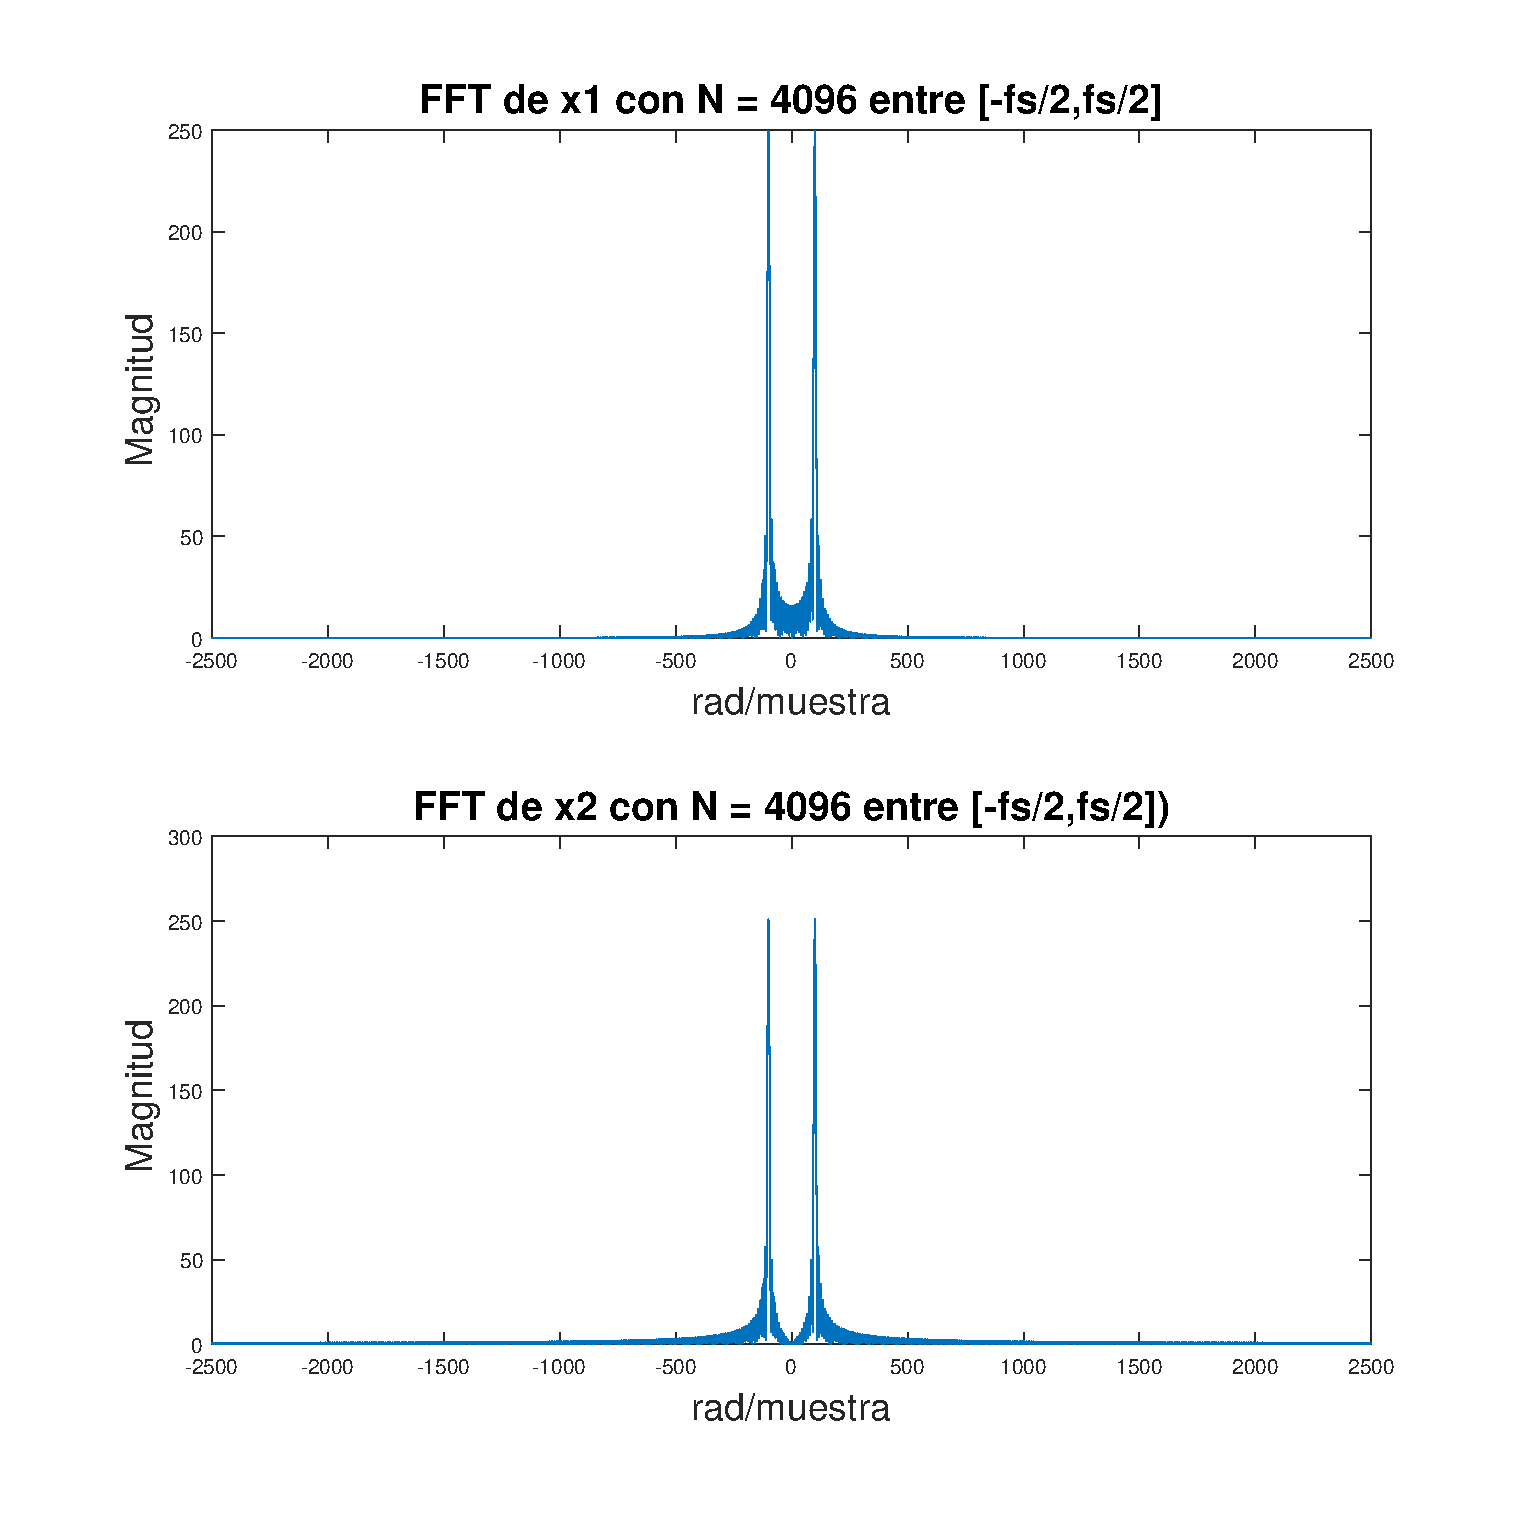
\includegraphics[scale = 0.6]{Figuras/p1_2-fs-medios.eps}
        \caption{Magnitud de la fft para las señales $x_1$ y $x_2$ entre   $[-\frac{fs}{2},\frac{fs}{2}]$ con N = 4096}
        \label{fs-medios}
    \end{figure}
    
        \begin{figure}[H]
        \centering
        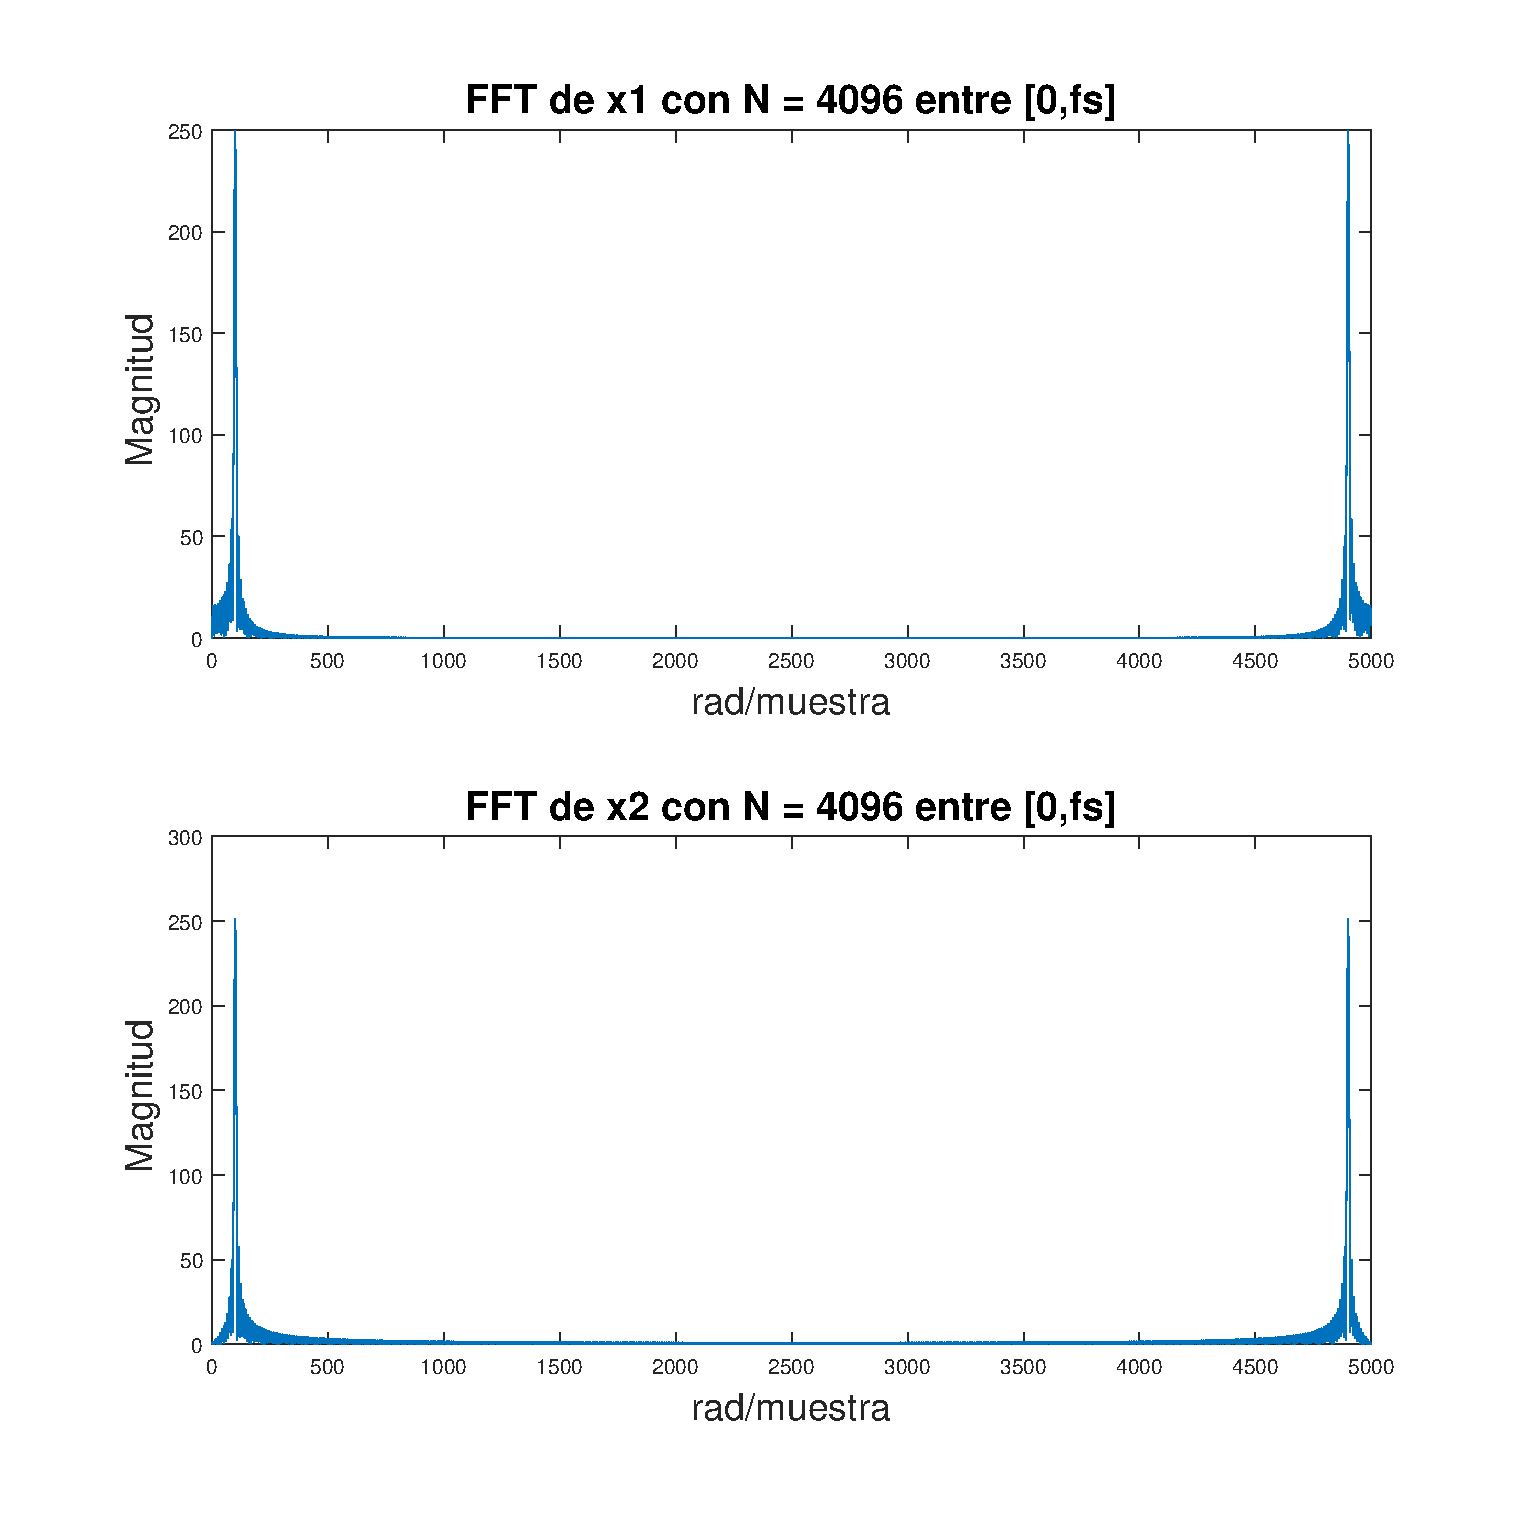
\includegraphics[scale = 0.6]{Figuras/p1_2-cero-fs-medio.eps}
        \caption{Magnitud de la fft para las señales $x_1$ y $x_2$ entre   $[0,\frac{fs}{2}]$ con N = 4096}
        \label{cero-fs-medio}
    \end{figure}


En las gráficas de ambas figuras se puede observar que el espectro tiene una amplitud de 250, lo que tiene sentido ya que este valor corresponde a la suma de todas las muestras y en este caso eran señales de 500 muestras, esto además de el factor de $\frac{1}{2}$ asociado a la transformada de Fourier de señales sinusoidales hace que los resultados obtenidos coincidan con los esperados.

\item Se obtiene la DFT de cada una de las señales anteriores, $x_1 $ y $x_2$,  para  valores de $N = 256$, $N = 500$ y $N = 2048$, luego se obtienen gráficos de magnitud $v/s$ Frecuencia además de la parte real y parte imaginaria $v/s$ frecuencia. Las gráficas obtenidas para $x_1$ se muestran en la figura \ref{x1} mientras que las correspondientes a la señal $x_2$ se encuentran en la figura \ref{x2}

\begin{figure}[H]
    \centering
    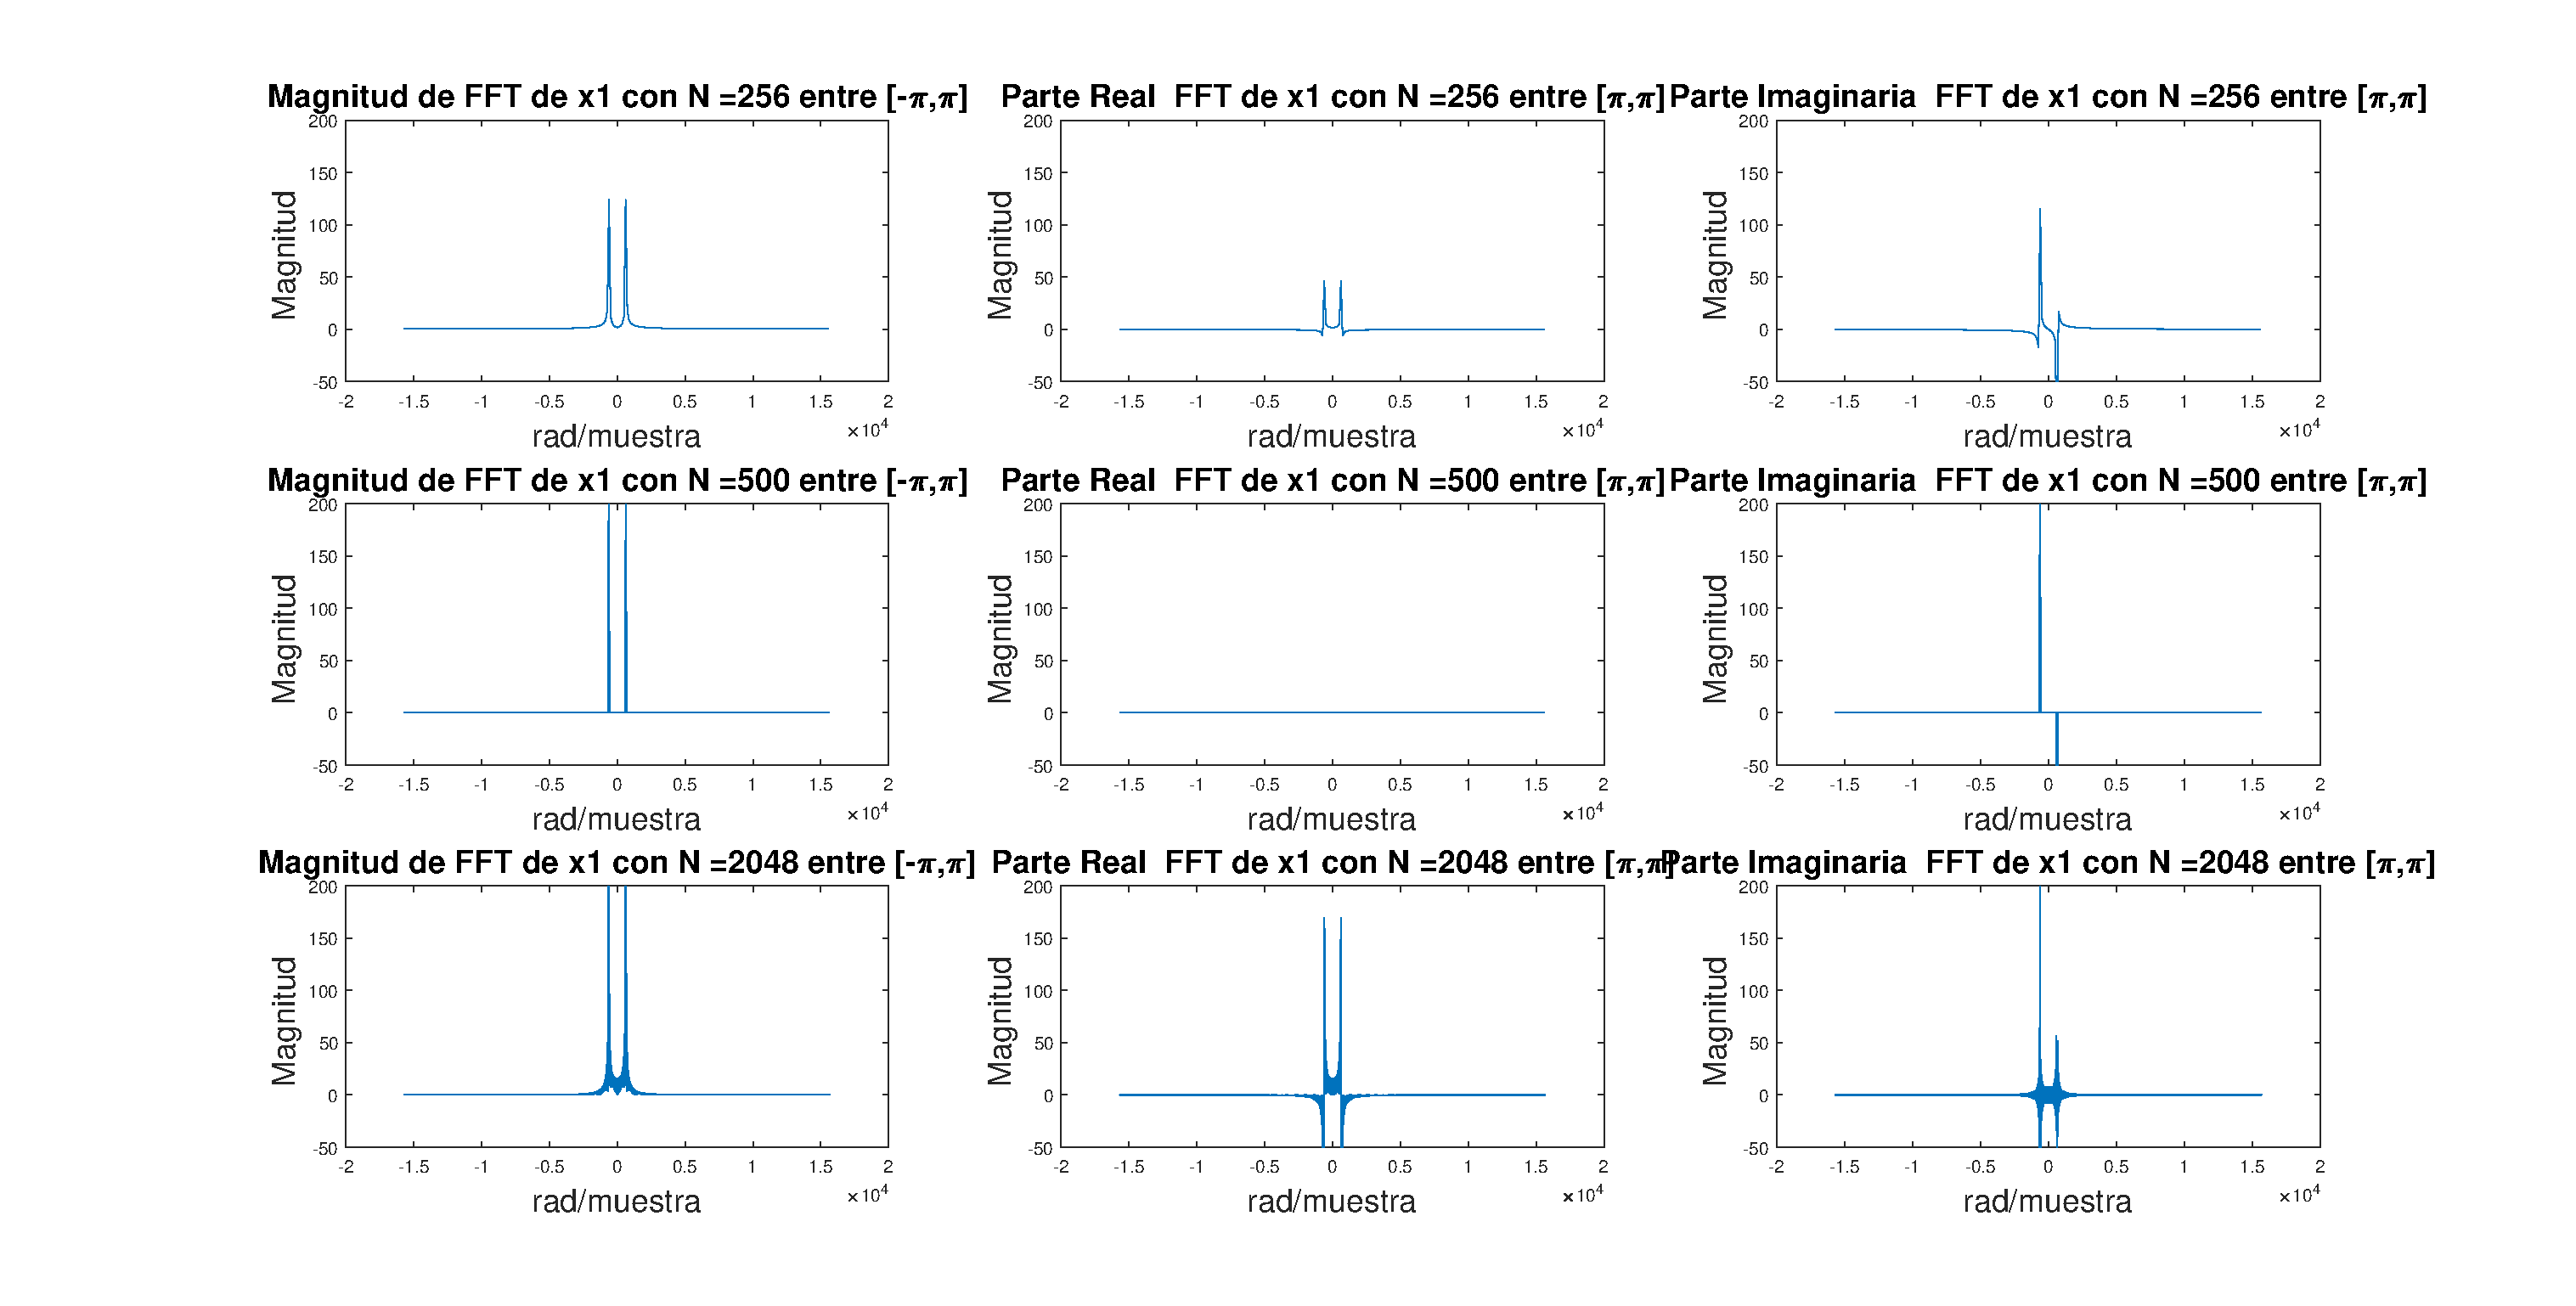
\includegraphics[scale = 0.3]{Figuras/p1_3-x1.eps}
    \caption{Magnitud y partes real e imaginaria de la señal $x_1 = sin(\omega t)$ para $N = 256,500,2048$}
    \label{x1}
\end{figure}

\begin{figure}[H]
    \centering
    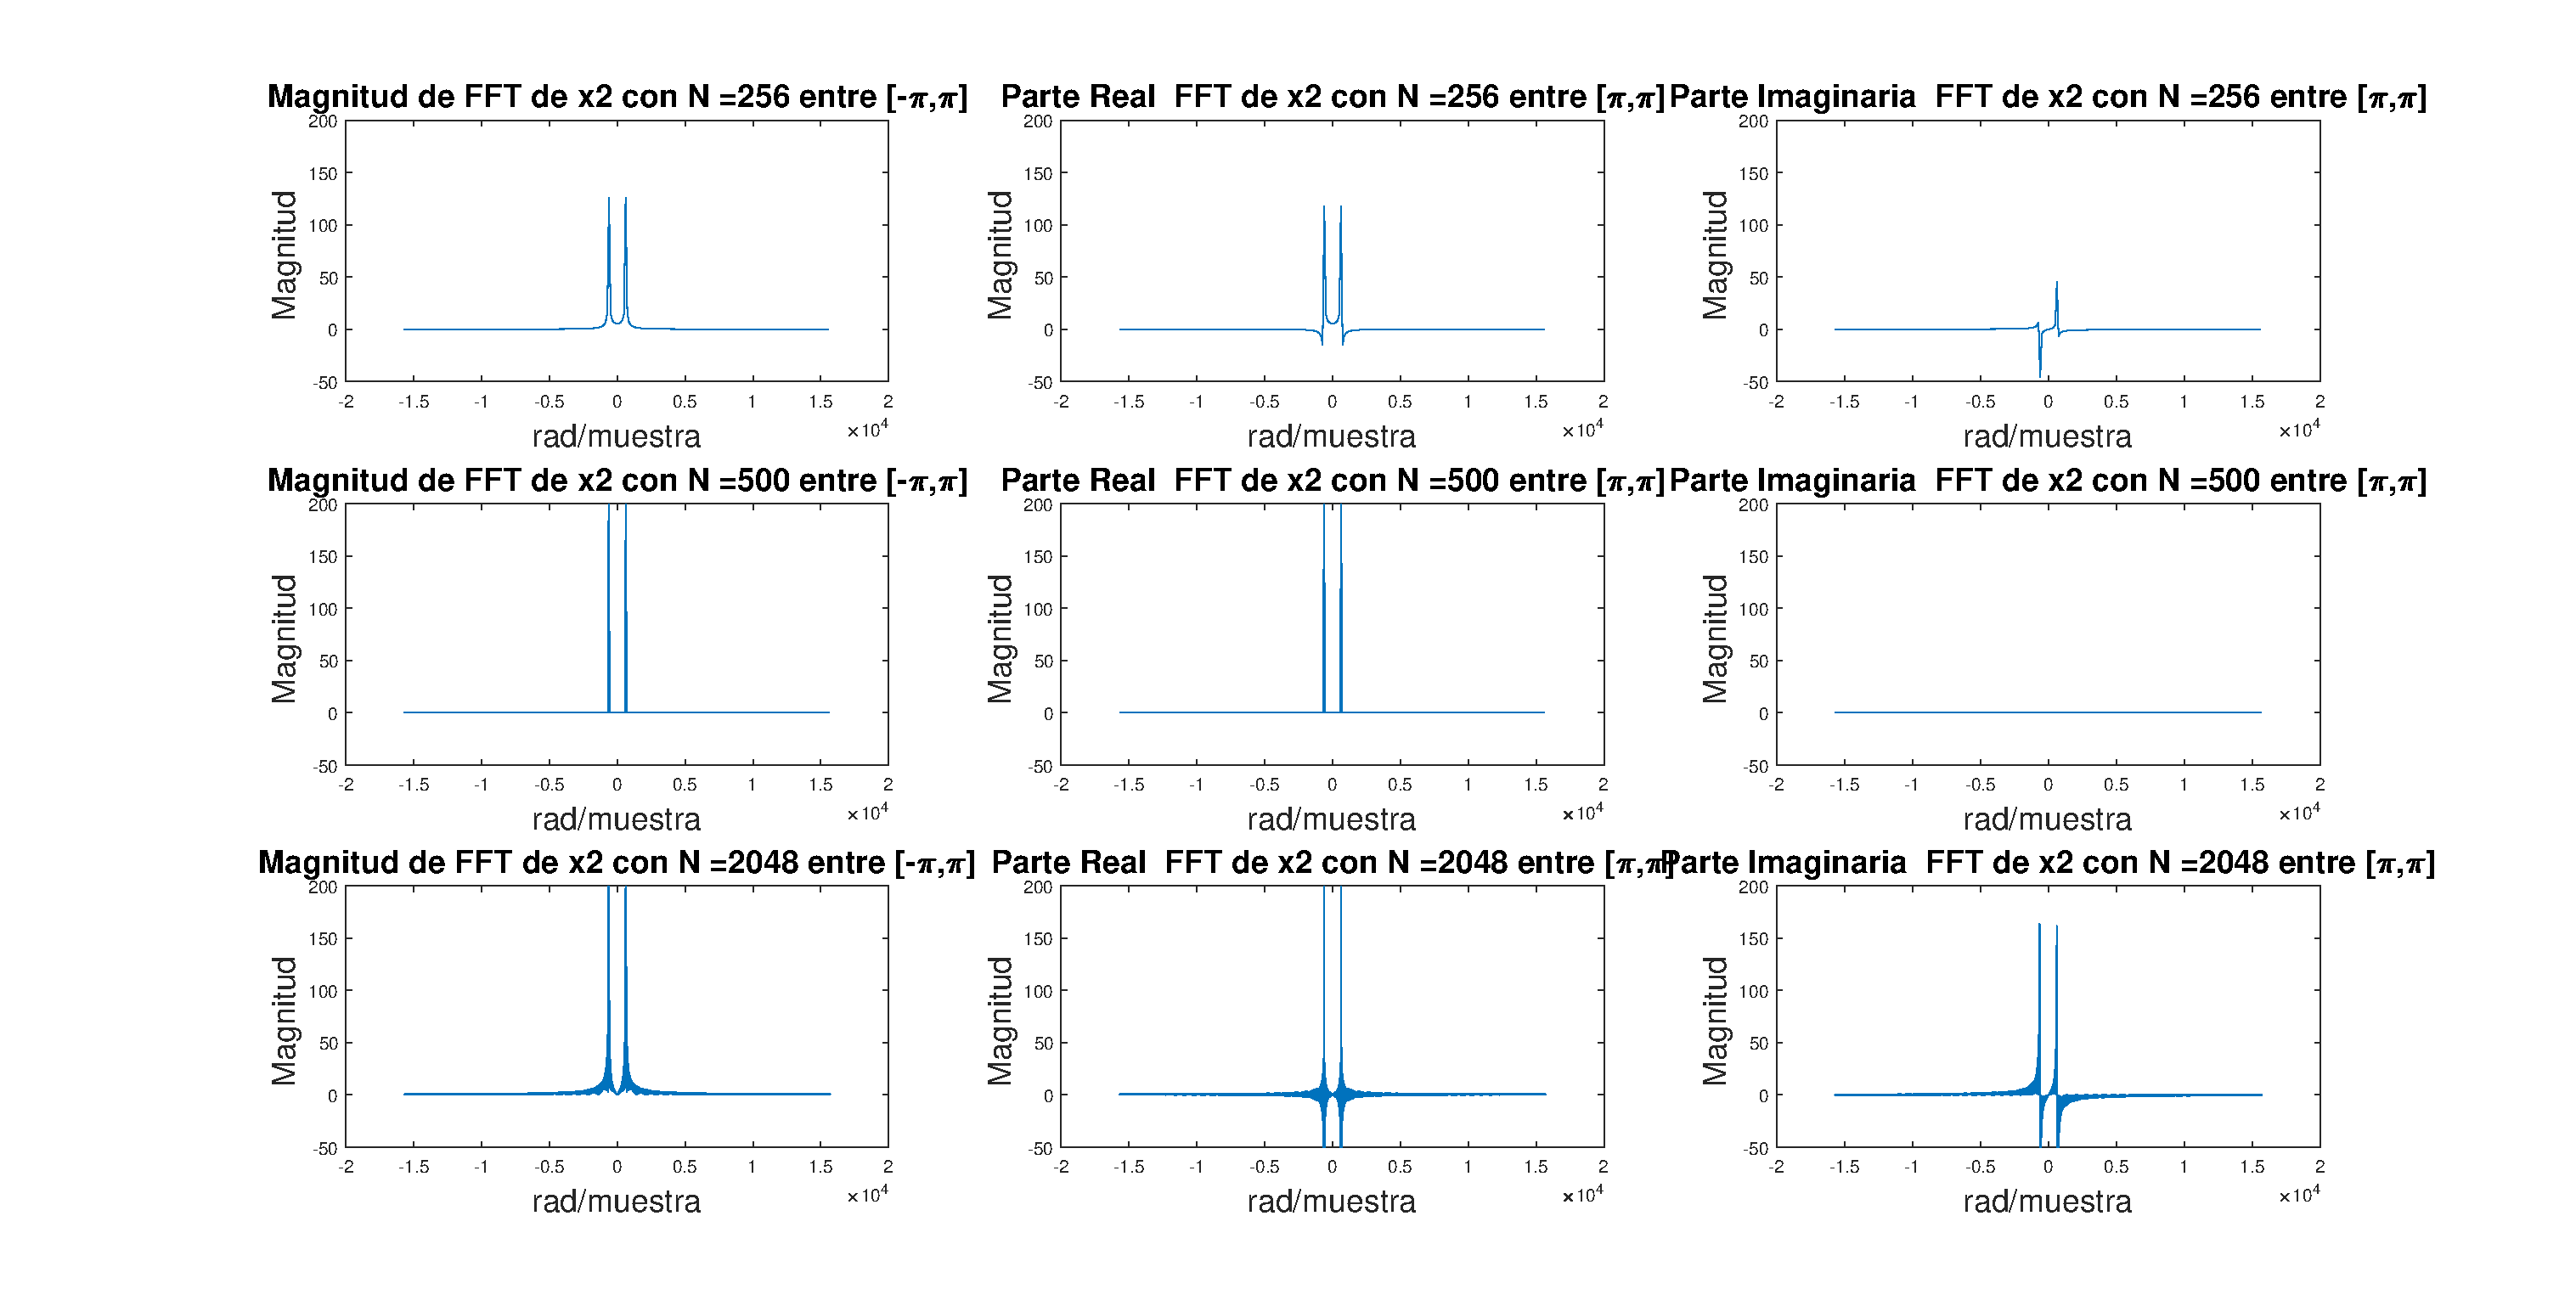
\includegraphics[scale = 0.3]{Figuras/p1_3-x2.eps}
    \caption{Magnitud y partes real e imaginaria de la señal $x_2 = cos(\omega t)$ para $N = 256,500,2048$}
    \label{x2}
\end{figure}

De las gráficas anteriores se puede concluir que el valor de N más apropiado es de 500, ya que los resultados obtenidos son los espectros más prolijos y cercanos a lo que se espera teóricamente de la transformada de ambas señales en caso de ser infinitas, esto se debe a que el $N=500$ permite que los bines de frecuencia  coincidan con las señales $sinc $ asociadas a las ventanas usadas en la transformación. 

En caso que se busque un resultado cercano para señales finitas el valor que proporciona mejores resultados es de $N = 2048$, en las graficas obtenidas con este N se pueden apreciar los lóbulos laterales que se generan por las ventanas asociadas a la transformación.





\end{enumerate}